%
% underdetermined.tex -- underdetermined solution
%
% (c) 2019 Prof Dr Andreas Müller, Hochschule Rapperswil
%
\documentclass[tikz,12pt]{standalone}
\usepackage{amsmath}
\usepackage{times}
\usepackage{txfonts}
\usepackage{pgfplots}
\usepackage{csvsimple}
\usetikzlibrary{arrows,intersections,math}
\begin{document}
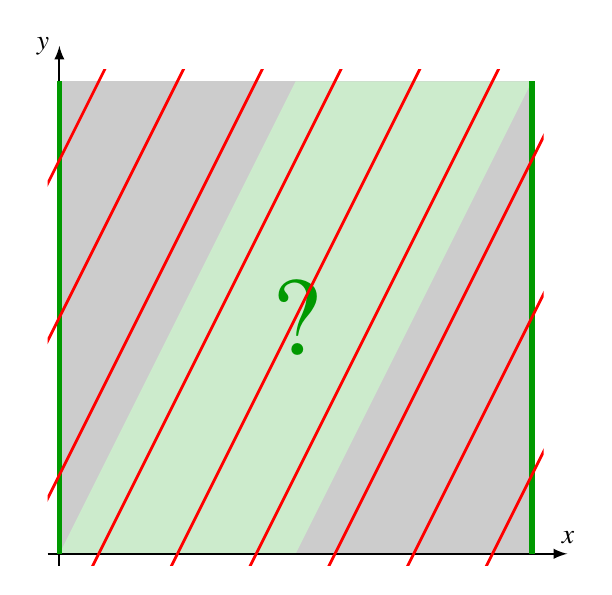
\begin{tikzpicture}[>=latex,scale=1.5]

\definecolor{darkgreen}{rgb}{0,0.6,0}

\fill[color=gray!40] (0,0)--(4,0)--(4,4)--(0,4)--cycle;
\fill[color=darkgreen!20] (0,0)--(2,0)--(4,4)--(2,4)--cycle;
\draw[->,line width=0.7pt] (-0.1,0)--(4.3,0) coordinate[label={$x$}];
\draw[->,line width=0.7pt] (0,-0.1)--(0,4.3) coordinate[label={left:$y$}];
\draw[color=darkgreen,line width=2pt] (0,0)--(0,4);
\draw[color=darkgreen,line width=2pt] (4,0)--(4,4);
\node[color=darkgreen,scale=4] at (2,2) {?};
\begin{scope}
\clip (-0.1,-0.1) rectangle (4.1,4.1);
\foreach \c in {-2,-1.333333,...,4.2}{
        \draw[color=red,line width=1pt] ({\c},-0.6666)--({\c+4},7.3333);
}
\end{scope}

\end{tikzpicture}
\end{document}

